%!TEX root = ../GLM_Becerra_Lopez.tex

\section{Resultados}
\label{sec:resultados}

En la figura \ref{fig:comp_pooling_resids} se muestran los residuales del modelo en el eje $y$, y en el eje $x$ se muestra el índice de la observación, donde las observaciones están ordenadas de acuerdo a código postal. Es evidente un patrón, que viene de la correlación entre las observaciones que existe dentro de cada código postal.

\begin{figure}[H]
    \centering
    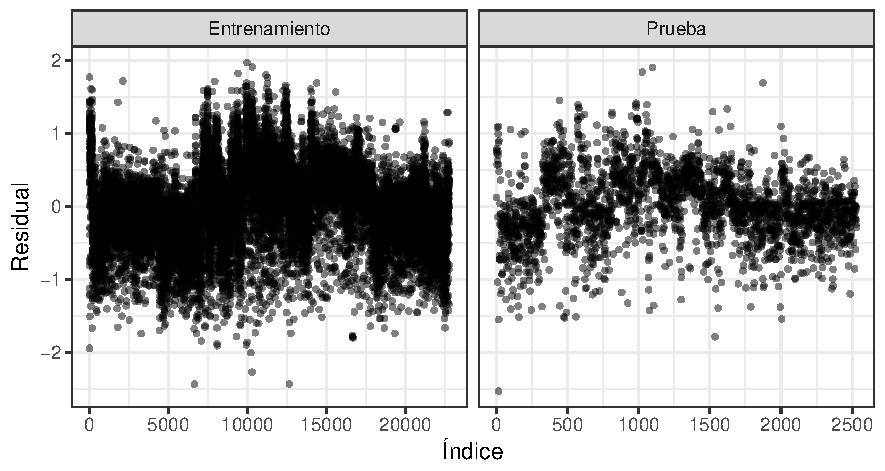
\includegraphics[width=0.8\textwidth]{images/comp_pooling_resids.pdf}
    \caption{Residuales de modelo de unidades iguales}
    \label{fig:comp_pooling_resids}
\end{figure}

En la figura \ref{fig:comp_pooling_obs_vs_pred} se puede ver para cada observación el valor observado contra el valor ajustado. Se aprecia una varianza considerablemente grande y que además en los valores pequeños, el modelo tiende a sobreestimar, mientras que en valores grandes pasa lo contrario.

\begin{figure}[H]
    \centering
    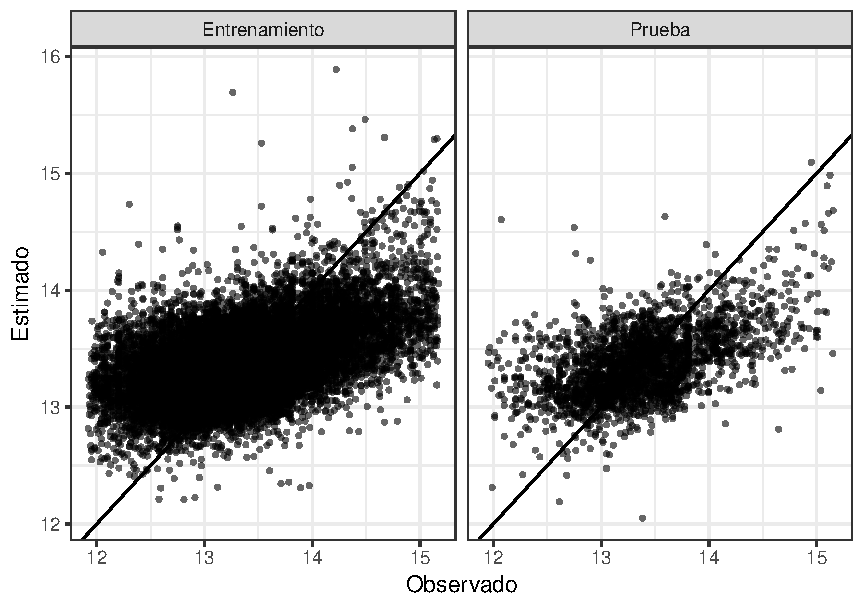
\includegraphics[width=0.8\textwidth]{images/comp_pooling_obs_vs_pred.pdf}
    \caption{Ajustado contra observado en modelo de unidades iguales}
    \label{fig:comp_pooling_obs_vs_pred}
\end{figure}


En la figura \ref{fig:no_pooling_resids} se pueden ver los residuales del modelo de unidades independientes. Se puede ver que ya no se ven los patrones tan evidentes del código postal como en el modelo de unidades iguales.

\begin{figure}[H]
    \centering
    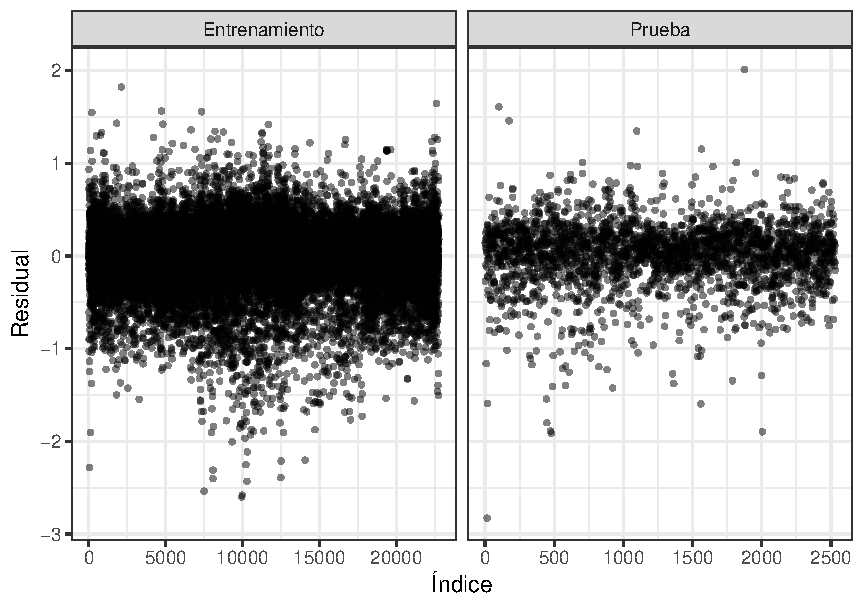
\includegraphics[width=0.8\textwidth]{images/no_pooling_resids.pdf}
    \caption{Residuales de modelo de unidades independientes}
    \label{fig:no_pooling_resids}
\end{figure}

En la figura \ref{fig:no_pooling_obs_vs_pred} se muestra el valor observado contra el valor ajustado

\begin{figure}[H]
    \centering
    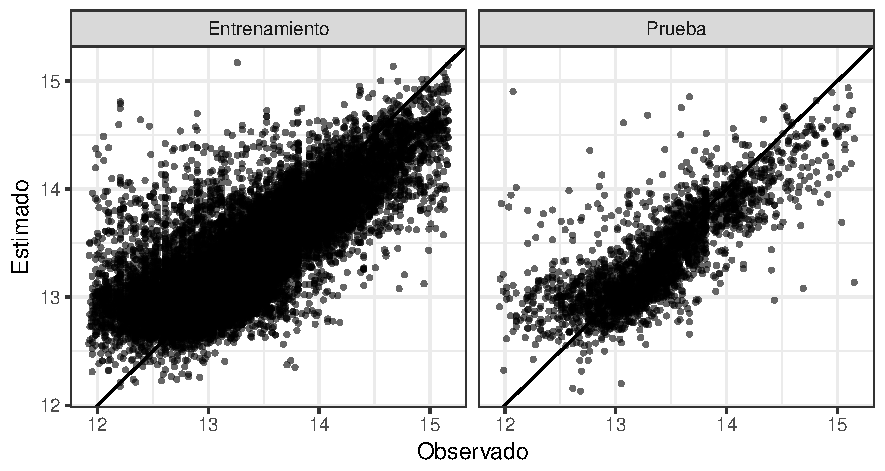
\includegraphics[width=0.8\textwidth]{images/no_pooling_obs_vs_pred.pdf}
    \caption{Valor ajustado contra observado en modelo de unidades independientes}
    \label{fig:no_pooling_obs_vs_pred}
\end{figure}

\begin{figure}[H]
    \centering
    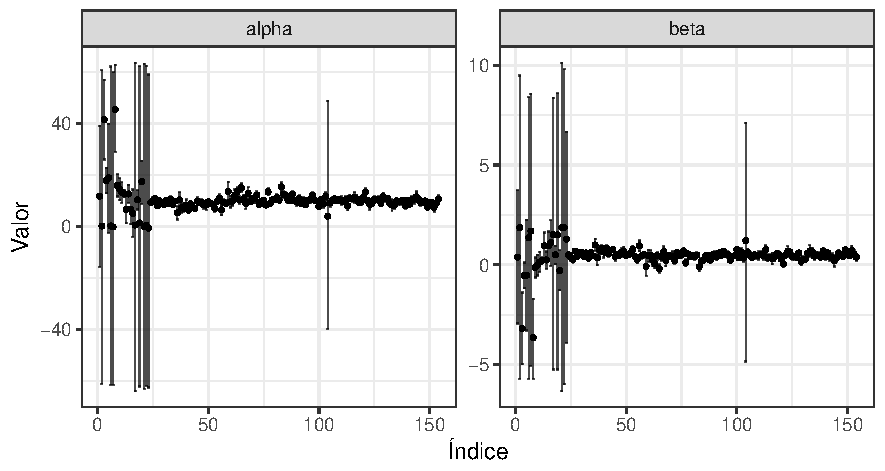
\includegraphics[width=0.9\textwidth]{images/no_pooling_param_values.pdf}
    \caption{Valor e intervalos de probabilidad de parámetros de modelo de unidades independientes}
    \label{fig:no_pooling_param_values}
\end{figure}




En la figura \ref{fig:three_levels_resids} se pueden ver los residuales del modelo multinivel.


\begin{figure}[H]
    \centering
    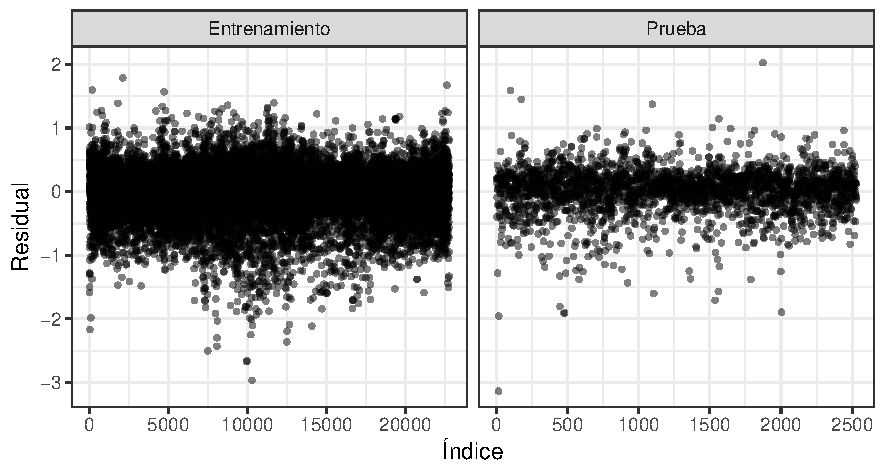
\includegraphics[width=0.8\textwidth]{images/three_levels_resids.pdf}
    \caption{Residuales de modelo multinivel}
    \label{fig:three_levels_resids}
\end{figure}

\begin{figure}[H]
    \centering
    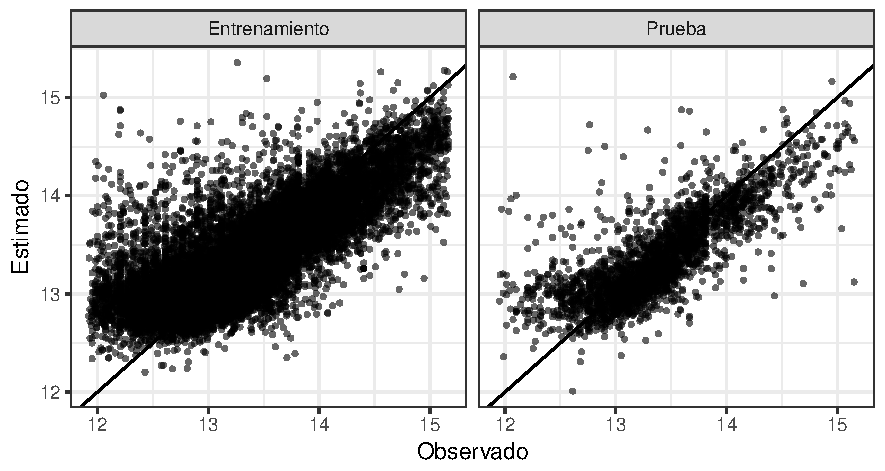
\includegraphics[width=0.8\textwidth]{images/three_levels_obs_vs_pred.pdf}
    \caption{Valor ajustado contra observado en modelo multinivel}
    \label{fig:three_levels_obs_vs_pred}
\end{figure}

\begin{figure}[H]
    \centering
    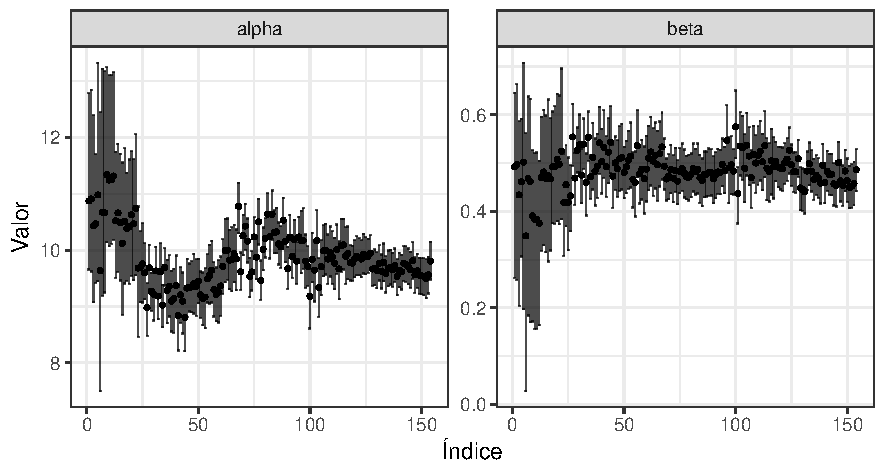
\includegraphics[width=0.9\textwidth]{images/three_levels_param_values.pdf}
    \caption{Valor e intervalos de probabilidad de parámetros de modelo multinivel}
    \label{fig:three_levels_param_values}
\end{figure}

\subsection{Comparación de modelos}

En esta subsección se comparan los modelos.
